\documentclass[a4paper,12pt]{article}
\usepackage{graphicx}
\usepackage{float} 
\usepackage{subfigure}

\begin{document}

\title{Evaluation on Prevalent FOND Planning Techniques\\
\large Honours Thesis }

\author{Yifan Wang \\
\textbf{Supervisor: }Sebastian Sardina\\
{\small RMIT University}
}

\date{October, 2020}
\maketitle

%\tableofcontents

\section{Introduction}


\section{Literature review}

\subsection{About Planning}
\subsubsection{Automated Planning}
AI planning(automated planning) is the model-based approach to autonomous behaviour and an important branch of artificial intelligence. The two main motivations for AI planning research are that planning acts an important part in the computing area of artificial intelligence and plans are desirable to be created automatically in some cases needed in many different areas of humanity\cite{key1}. Planning can be classified hinge on whether and how they can be constructed to accomplish in various plan domains: domain-specific planners, domain-independent planners, and domain-configurable planners. The domain-independent planning, namely the classical planning has been dominated by research for almost the entire time that automated planning exists\cite{key1}. Most research has focused on classical planning due to the huge difficulties of developing a domain-independent planner that would work well in all planning domains. Classical planning needs to content the following set of underlying presumptions: the planner has a limited set of fully observable states, namely, the planner has intact knowledge about the states, effects are deterministic for all actions after execution, and the solution to a planning problem is a linearly ordered finite sequence of actions\cite{key5}. Classical planning is not applicable to solve a number of realistic world problems. Actually in the real world, some effects after the accomplishment of actions are non-deterministic. For instance, the effect of flipping a coin is non-deterministic because the side of the coin facing up could be heads or tails after the flipping action. Fortunately, automated-planning research is moving away from the restrictions of classical planning, and planning in non-deterministic and probabilistic domains is the trend of automated-planning \cite{key1}. One of the important motivations for us to study FOND(Fully observable non-deterministic) planning rather than classical planning is to solve some more practical problems. In planning, each action must have its corresponding effects. Conditional effects are effects which are applied whenever a given condition holds. One effect may have numbers of different but similar conditions, which will generate abounding actions, but we intend to have less actions as we can. Consequently, we use conditional effects to reduce the number of actions. For example, the action – ‘move the cup with water’ and the action – ‘move the empty cup’ are similar, we can reduce two actions into one simple action – ‘move the cup’ by adding conditional effects. Combining FOND planning and conditional effects can diminish the size of solutions for planning problems, this is the other one important motivation of our research. We will discuss some of the state-of-the-art of FOND planner in the next section, only one planner(PRP) has the support for conditional effects so far but the approach is complicated to implement. One more important motivation of our research is to fill the gap in the field of one other FOND planner(FOND-SAT) with the support for conditional effects. Hence, we focus our research on FOND planning in the general direction, and the goal of our research in a specific direction is to combine the SAT-based planner with conditional effects. We will discuss more specific details in the following sections.

\subsubsection{FOND Planning}
FOND planning is an extension of classical planning in which actions are non-deterministic and leads to a series of possible effects, and the effects are able to be observed by the agent\cite{key11}. In classical planning, the solution of a planning problem is a series of sequential actions. In FOND planning, there exists non-deterministic actions, the achievable executions form a tree, and policies have to decide the proper actions for every node of the tree. So the solution of a FOND planning problem is a policy in which a state corresponds to a proper action, in this way the agent finally achieves the goal state. There are generally three kinds of solutions: weak, strong and strong cyclic. For weak solutions, goals that are possible but not certain to be achieved. For strong solutions, that are certain to reach the goals. For strong cyclic solutions, that are certain to reach the goal under a “fairness” presumption\cite{key6}. Their execution can bring an infinite series of states, for example, the execution can cycle eternally. Nevertheless, this happens only if several actions are executed infinitely often in a given state and other actions that lead to the goal never occur. We call these types of executions “unfair”. The solutions of classical planning are the strong solutions. But for FOND planning, the practical solutions are always strong cyclic solutions\cite{key11}. In this section, we will review the basic concepts in planning and several planners which are the state of art of FOND planning.


\subsubsection{STRIPS}
The STRIPS(STanford Research Institute Problem Solver) is an ancient but significant problem-solving program that works by executing a domain and problem to find a goal and is the basis and predecessor of PDDL(Planning Domain Definition Language)\cite{key2}. With STRIPS, we are able to describe the world by providing objects, actions, preconditions, and effects.
\subsubsection{PDDL}
PDDL is able to generate procedures involving iteration (or recursion) and conditional branching that STRIPS are unable to handle. PDDL is the standard encoded language for classical planning tasks as well as the official language of International Planning Competition (IPC)\cite{key12}. The existing benchmarks of planning problems are writed by PDDL, like \textbf{search}, \textbf{tireworld} and so on. There are two types of files in PDDL, one is the domain file and another one is the problem file. In the domain file, we describe the predicates and actions. In the problem file, we give the initial state and goal state. The requirements of the domain file give us support for conditional effects of an action.
\begin{figure}[H]
\centering  
\subfigure[Domain file]{
\label{Fig.sub.1}
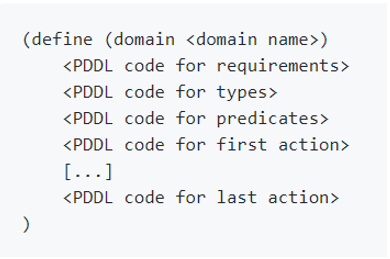
\includegraphics[width=0.45\textwidth]{domain}}
\subfigure[Problem file]{
\label{Fig.sub.2}
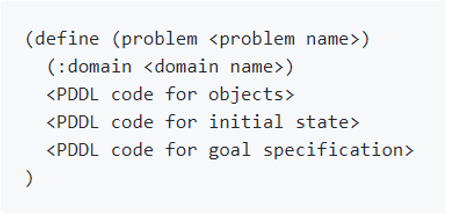
\includegraphics[width=0.45\textwidth]{problem}}
\caption{PDDL files}
\label{Fig.main}
\end{figure}
\subsubsection{ SAS+}
 SAS+ is an extension of the STRIPS formalism to include functional state variables, which map to objects of the planning problem instead of the binary set \{true, false\}\cite{key3}. SAS+ formalism is always using for SAT based planning problem, resulting in an encoding that is both more
compact and efficient for planning\cite{key16}.



\subsection{FOND Planning Techniques}

\subsubsection{MBP}

\subsubsection{PRP}
PRP planner is the state of the art of FOND planning developed for both FOND and online probabilistic planning problems by build a strong cyclic solution, not only generates solutions up to several orders of magnitude faster but generates policies several orders of magnitude smaller than the most advanced FOND planner before, FIP \cite{key7}. To find a strong cyclic plan, PRP uses the approach that repeat finding weak plans using the all outcomes determinization until find a strong cyclic plan. Rather than using the intact state, using regressed partial state and combine the state-action pair with the distance to the found weak plan’s goal is the core aspect of PRP algorithm. Focusing on what related to succeed in weak plans is a core direction of PRP's success\cite{key9}.




\begin{subsubsection}{{\footnotesize MY}ND}
{\scriptsize MY}ND planner is the other branch of FOND planers that relying on explicit AND/OR graph search. Strong cyclic plans are  exported in the form of a states-action pairs by the planner, which is then interpreted by the execution simulator\cite{key10}.  As a contrast, classical planning performs faster when most actions are deterministic, but {\scriptsize MY}ND planner show better overall performance both in deterministic and non-deterministic problems and never ends up in a dead-end\cite{key10}.
\end{subsubsection}

\begin{subsubsection}{SAT-based}
Classic FOND planners such as PRP scale up best to problem size and even policy size, but they may propagate and generalize dead-ends because of not having to produce and abandon each of misleading weak plans\cite{key8}. SAT approach to FOND planning relies on compact, polynomial encodings, which have an aptitude for handling richer forms of non-determinism because it has the ability to reason in parallel about the diverse branches of futures produced by non-deterministic actions\cite{key8}. There is still no research has been done on SAT-based FOND planner with conditional effects at present, and this is one of significant gap in FOND planning. 

\end{subsubsection}







\section{Experiment}


\section{Evaluation}


\bibliographystyle{ieeetr}
% there are various bibliography styles you can set

\bibliography{References}
% this tells latex to generate the reference list, using the references.bib file of references.
% you will need to do pdflatex <tex filename>; then bibtex <tex filename without extension>;
% pdflatex <tex filename> again twice. then you have a formatted pdf.

\end{document}
